\documentclass[preview]{standalone}
%\usepackage[dvipdfm]{geometry}
\usepackage{ctex}
%graphics
\usepackage{xcolor}
\usepackage{tikz}
\usetikzlibrary{shapes.geometric, shapes.multipart, arrows, arrows.meta,calc, through,intersections, circuits.logic.US}
\usepackage[caption=false,font=footnotesize]{subfig}

\begin{document}
    

\begin{figure}[!t]
\centering

\subfloat[逻辑网络]{
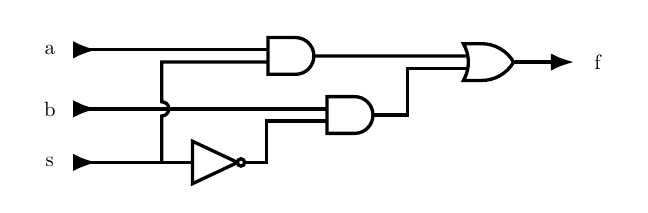
\begin{tikzpicture}[transform shape, scale=0.75, circuit logic US, every node/.style={very thick, minimum size=0.75cm}, very thick]

\node(o1)[or gate, point right]  at (6,3){};
\draw[>=Latex, ->] (o1.output) -- +(1,0) node[right]{f};

\node (a1)[and gate, point right] at ($(o1.input 1) - (3,0)$) {};
\node (a2)[and gate, point right] at ($(o1.input 1) - (2,1)$) {};

\draw (o1.input 1) -- (a1.output);
\draw (o1.input 2) -- ++(-1,0) |- (a2.output);

\node (n1)[not gate, point right] at ($(a2.input 2) - (2,0.7)$) {};
\draw (a2.input 2) -- ++(-1, 0) |- (n1.output);

\coordinate (pivot) at ($(n1.input) - (2,0)$);

\begin{scope}[>=Latex]
\draw[>-] (n1.input -| pivot) node(s)[left]{s} --(n1.input);
\draw[>-] (a2.input 1 -| pivot) node(b)[left]{b} --(a2.input 1);
\draw[>-] (a1.input 1 -| pivot) node(a)[left]{a} --(a1.input 1);
\end{scope}

\coordinate (p2) at ($(n1.input) - (0.5, 0)$);
\coordinate (arcc) at (p2 |- b);
\draw (p2) -- ($(arcc) - (0, 0.12) $) arc[start angle=-90, end angle=90, radius=0.12] |- (a1.input 2);
\end{tikzpicture}
}
\subfloat[DAG 结构]{
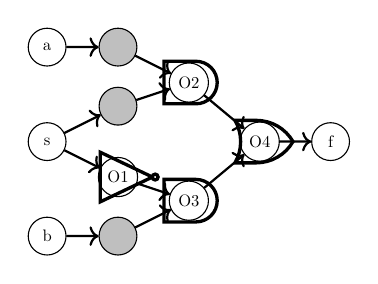
\begin{tikzpicture}[transform shape, circuit logic US, every node/.style={minimum size=.8cm}, scale=0.6]
 \node(b)[circle, draw] at (0,1) {b};
\node(s)[circle, draw] at (0,3) {s};
\node(a)[circle, draw] at (0,5) {a};

\node(7)[circle, draw, fill=lightgray] at (1.5,1) {};
\node(O1)[circle, draw] at (1.5,2.25) {O1};
\node(5)[circle, draw, fill=lightgray] at (1.5,3.75) {};
\node(4)[circle, draw, fill=lightgray] at (1.5,5) {};

\node(O3)[circle, draw] at (3,1.75) {O3};
\node(O2)[circle, draw] at (3,4.25) {O2};

\node(O4)[circle, draw] at (4.5,3) {O4};
\node(f)[circle, draw] at (6,3) {f};

\draw[->, thick] (b) -- (7);
\draw[->, thick] (s) -- (O1);
\draw[->, thick] (s) -- (5);
\draw[->, thick] (a) -- (4);
\draw[->, thick] (7) -- (O3);
\draw[->, thick] (O1) -- (O3);
\draw[->, thick] (5) -- (O2);
\draw[->, thick] (4) -- (O2);
\draw[->, thick] (O2) -- (O4);
\draw[->, thick] (O3) -- (O4);
\draw[->, thick] (O4) -- (f);


\node[not gate, point right, minimum size=.9cm, very thick] (and1) at (O1){};
\node[and gate, point right, minimum size=.9cm, very thick] (and1) at (O2){};
\node[and gate, point right, minimum size=.9cm, very thick] (and1) at (O3){};
\node[or gate, point right, minimum size=.9cm, very thick] (and1) at (O4){};
\end{tikzpicture}
}

\subfloat[分层DAG图]{
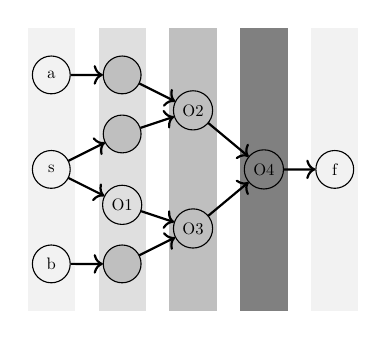
\begin{tikzpicture}[transform shape, circuit logic US, every node/.style={minimum size=.8cm}, scale=0.6]
\fill[color=lightgray!20] (-0.5,0) rectangle (0.5,6);
\fill[color=lightgray!50] (1,0) rectangle (2,6);
\fill[color=lightgray] (2.5,0) rectangle (3.5,6);
\fill[color=gray] (4,0) rectangle (5,6);
\fill[color=lightgray!20] (5.5,0) rectangle (6.5,6);

\node(b)[circle, draw] at (0,1) {b};
\node(s)[circle, draw] at (0,3) {s};
\node(a)[circle, draw] at (0,5) {a};

\node(7)[circle, draw, fill=lightgray] at (1.5,1) {};
\node(O1)[circle, draw] at (1.5,2.25) {O1};
\node(5)[circle, draw, fill=lightgray] at (1.5,3.75) {};
\node(4)[circle, draw, fill=lightgray] at (1.5,5) {};

\node(O3)[circle, draw] at (3,1.75) {O3};
\node(O2)[circle, draw] at (3,4.25) {O2};

\node(O4)[circle, draw] at (4.5,3) {O4};
\node(f)[circle, draw] at (6,3) {f};



\draw[->, thick] (b) -- (7);
\draw[->, thick] (s) -- (O1);
\draw[->, thick] (s) -- (5);
\draw[->, thick] (a) -- (4);
\draw[->, thick] (7) -- (O3);
\draw[->, thick] (O1) -- (O3);
\draw[->, thick] (5) -- (O2);
\draw[->, thick] (4) -- (O2);
\draw[->, thick] (O2) -- (O4);
\draw[->, thick] (O3) -- (O4);
\draw[->, thick] (O4) -- (f);
\end{tikzpicture}
}
\hfil
\subfloat[电路布局]{
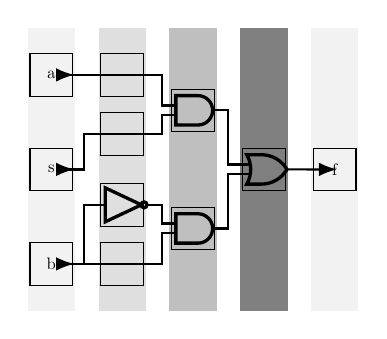
\begin{tikzpicture}[transform shape, circuit logic US, every node/.style={minimum size=0.9cm}, scale=0.6]
\fill[color=lightgray!20] (-0.5,0) rectangle (0.5,6);
\fill[color=lightgray!50] (1,0) rectangle (2,6);
\fill[color=lightgray] (2.5,0) rectangle (3.5,6);
\fill[color=gray] (4,0) rectangle (5,6);
\fill[color=lightgray!20] (5.5,0) rectangle (6.5,6);

\node(b)[draw] at (0,1) {b};
\node(s)[draw] at (0,3) {s};
\node(a)[draw] at (0,5) {a};

\node(7)[draw] at (1.5,1) {};
\node(O1)[draw] at (1.5,2.25) {};
\node(5)[draw] at (1.5,3.75) {};
\node(4)[ draw ] at (1.5,5) {};

\node(O3)[draw] at (3,1.75) {};
\node(O2)[draw] at (3,4.25) {};

\node(O4)[draw] at (4.5,3) {};
\node(f)[draw] at (6,3) {f};

\node[not gate, point right,  very thick] (not1) at ($(O1)-(0.1,0)$){};
\node[and gate, point right, very thick] (and1) at (O2){};
\node[and gate, point right, very thick] (and2) at (O3){};
\node[or gate, point right, very thick] (or1) at (O4){};

\begin{scope}[>=Latex, thick]
\draw[>-] ($(a) + (0.1,0)$) -- ++(2.25,0) |- (and1.input 1);
\draw[>-] ($(s) + (0.1,0)$) -- ++(0.6,0) -- ++(0,0.75) -- ++(1.65,0) |- (and1.input 2);
\draw[>-] ($(b) + (0.1,0)$) -- ++(0.6,0) coordinate (d) |- (not1.input);
\draw (d) -- ++(1.65,0) |- (and2.input 2);
\draw (not1.output) -- ++(0.3,0) |- (and2.input 1);
\draw(and1.output) -- ++(0.3,0) |- (or1.input 1);
\draw(and2.output) -- ++(0.3,0) |- (or1.input 2);
\draw[->] (or1.output) -- ($(f) + (0.05,0)$);
    
\end{scope}


%\draw[->, thick] (b) -- (7);
%\draw[->, thick] (s) -- (O1);
%\draw[->, thick] (s) -- (5);
%\draw[->, thick] (a) -- (4);
%\draw[->, thick] (7) -- (O3);
%\draw[->, thick] (O1) -- (O3);
%\draw[->, thick] (5) -- (O2);
%\draw[->, thick] (4) -- (O2);
%\draw[->, thick] (O2) -- (O4);
%\draw[->, thick] (O3) -- (O4);
%\draw[->, thick] (O4) -- (f);
\end{tikzpicture}
}

\end{figure}
\end{document}
